\documentclass[12pt]{article}
\usepackage[latin1,utf8]{inputenc}
\usepackage[brazil]{babel}
\usepackage{setspace}
\usepackage{boxedminipage}
\usepackage{latexsym}
\usepackage{multirow}
\usepackage[pdftex]{graphicx}
\usepackage{float}
\usepackage{url}
\usepackage{xcolor,listings}

%\setlength{\parskip}{0.1cm}
\setlength{\paperheight}{29.7cm}
\setlength{\textheight}{23.0cm}
\setlength{\textwidth}{16.5cm}
\setlength{\oddsidemargin}{0.0cm}
\setlength{\topmargin}{-1.0cm}
\pagestyle{empty}

% Custom colors
\usepackage{color}
\definecolor{deepblue}{rgb}{0,0,0.5}
\definecolor{deepred}{rgb}{0.6,0,0}
\definecolor{deepgreen}{rgb}{0,0.5,0}

\begin{document}

\lstset{language=python,
    keywordstyle=\color{deepblue}\bfseries,
    commentstyle=\color{deepgreen},
    stringstyle=\ttfamily\color{deepred!50!brown},
    breaklines=true,
    showstringspaces=false}
\lstset{literate=%
   *{0}{{{\color{red!20!violet}0}}}1
    {1}{{{\color{red!20!violet}1}}}1
    {2}{{{\color{red!20!violet}2}}}1
    {3}{{{\color{red!20!violet}3}}}1
    {4}{{{\color{red!20!violet}4}}}1
    {5}{{{\color{red!20!violet}5}}}1
    {6}{{{\color{red!20!violet}6}}}1
    {7}{{{\color{red!20!violet}7}}}1
    {8}{{{\color{red!20!violet}8}}}1
    {9}{{{\color{red!20!violet}9}}}1
}

\begin{center}
{\sf {\large Visão e Processamento de Imagens - Avaliação única -
    Parte II}}

\textbf{Preste atenção para as regras da prova}
\end{center}
1- O fonte latex (.tex) da prova será disponibilizado para facilitar
que você não tenha que copiar o enunciado das questões. Todas as questões
devem ser respondidas no mesmo arquivo.

\noindent 2- A prova é \textbf{individual}.  É permitido a consulta a
livros, apontamentos ou Internet, desde que devidamente referenciada.
Não é permitida a consulta a colegas, amigos, família, cachorro,
papagaio e etc. 

\noindent 3- A prova deve ser entregue diretamente no Paca, assim como
todos os códigos e imagens devem ser entregues no mesmo arquivo
comprimido.  \textbf{Duração da prova: 14 dias}.  

\noindent 4- Cada questão vale 20 pontos (pois são apenas 3 questões)
para a graduação e 15 pontos para a pós-graduação (pois são 4 questões). 
\bigskip

\begin{itemize}
\item[{\bf Q1.}] Para fazer esta questão, leia primeiro o artigo abaixo:
\begin{itemize}
\item \url{http://www.eecs.berkeley.edu/Pubs/TechRpts/2015/EECS-2015-85.pdf}
\end{itemize} 
\begin{itemize}
\item Faça um resumo do artigo de acordo com as indicações que deixei no paca (artigos sobre como fazer um resumo).
TODO

\item Implemente o método ELA (Error Level Analysis) em Python (apresente o 
\textbf{algoritmo} na prova e anexe o código em Python no arquivo zip).

Abaixo o trecho onde o algoritmo efetivamente foi implementado. O código completo está em \textbf{source/ela.py}.
    
\begin{lstlisting}[basicstyle=\ttfamily]
import os
from PIL import Image, ImageChops, ImageEnhance
from time import gmtime, strftime

# you can change the image directory here
HOAX_IMAGES = './HoaxImages/'

def check_image(img_path, scale=20.0, show=False):
    """ Compute the Error Level Analysis for the given image
    
    Save a copy of the given image changing its quality level,
    in our case 95%, and compute the difference between this 
    image over the original. In addition, a scale is also 
    applied to the final result for better viewing.
    
    References: 
    http://blackhat.com/presentations/bh-dc-08/Krawetz/Whitepaper/bh-dc-08-krawetz-WP.pdf
    http://www.eecs.berkeley.edu/Pubs/TechRpts/2015/EECS-2015-85.pdf
    """
    try:
        img = Image.open(img_path)
    except FileNotFoundError:
        print ("File '"+ img_path +"' not found.")
        return
    
    # check the image format for JPEG only
    if img.format is not 'JPEG':
        log(img_path + ' is not a JPEG file')
        return

    log("Image size "+ str(img.size[0]) + "x" + str(img.size[1]))
    short_file_name = os.path.splitext(img_path)[0]
    
    # save a copy of the image with a different inferior quality level rate
    resaved_path = short_file_name + '_resaved'
    img.save(resaved_path, 'JPEG', quality=95)
    resaved_img = Image.open(resaved_path)
    
    # compute the difference between the given image and the image
    # generated applying a scale to increase the brightness
    ela_img = ImageChops.difference(img, resaved_img)
    ela_img = ImageEnhance.Brightness(ela_img).enhance(scale)
    ela_img.save(short_file_name + '_ela.png')
    if (show):
        ela_img.show()
    
    os.remove(resaved_path)
\end{lstlisting}

\item Teste seu algoritmo com as imagens que deixei no paca para este exercício. 
Quantas imagens seriam consideradas modificadas por esse método? Comente o resultado,
comparando com a sua intuição.
Uma vez submetida a imagem ao Error Level Analysis, pode-se perceber pelo resultado que 
a região manipulada terá um nível de erro diferente do que as regiões não manipuladas. Logo, 
o nível de erro irá expor a região manipulada rotulando as regiões com maior alteração após
a imagem ser salva com um nível de qualidade inferior (Krawetz).

\end{itemize}
%
%
%
\item[{\bf Q2.}] Esta questão refere-se à transformada de Fourier.
\begin{itemize}
\item Encontre a transformada de Fourier da função:
\begin{eqnarray*}
f(x) = \left\{ \begin{array}{rl} 
 7 &\mbox{ if $-5 < x < 5$} \\
 0 &\mbox{ caso contrário}
       \end{array} \right.
\end{eqnarray*}
\item Encontre a transformada de Fourier da função $ g(x) = f(x)\cos
   \omega_0 x$, sabendo que a transformada de Fourier de $f(x)$ é dada
   por $F(\omega)$
\item Ache a inversa da transformada de Fourier de $G(\omega) =
  20\frac{\sin 5\omega}{5\omega}e^{-3\omega i}$
\item Calcule a DFT do sinal $f = \{1,3,5,3,1\}$
\end{itemize}
%
%
%
\item[{\bf Q3.}] 
\begin{itemize}
\item Calcule (apresente os cálculos) dos descritores de Fourier das
  figuras 1a e 1b. Lembre-se que os pontos da
  borda do quadrado serão representados por pontos no plano de
  Argand-Gauss. Isto é, cada ponto no plano passa a ser um número
  complexo e a borda passa a ser um vetor de pontos complexos, como
  num sinal, mas com valores complexos.
\item Para confirmar que seus cálculos estão corretos, implemente um
  programa em Python que receba como entrada um vetor de números
  complexos (que são as coordenadas das bordas) e retorne os
  descritores de Fourier do vetor de entrada. Você pode usar as
  funções fornecidas pela biblioteca NUMPY para facilitar a
  programação. 
\item Para reconstruir a curva, faça uma função que receba um vetor
  com os descritores de Fourier, um número $N$ de descritores a serem
  usados e grafique os pontos num plano cartesiano (para fazer a mesma 
figura que fizemos nos slides das aulas 15 e 16.
\end{itemize}
\begin{figure}[htb]
\centering
\begin{minipage}[b]{0.45\textwidth}
	\centering
        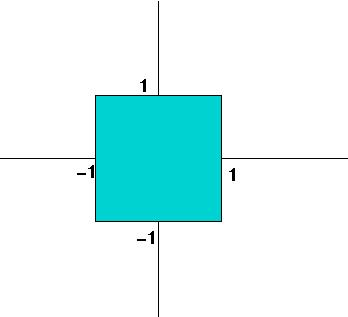
\includegraphics[scale=0.2]{Q3Images/square1.jpg} 
	\centerline{\label{fig1a} \small (1a) Quadrado de lado 1}
\end{minipage}
\begin{minipage}[b]{0.45\textwidth}
	\centering
        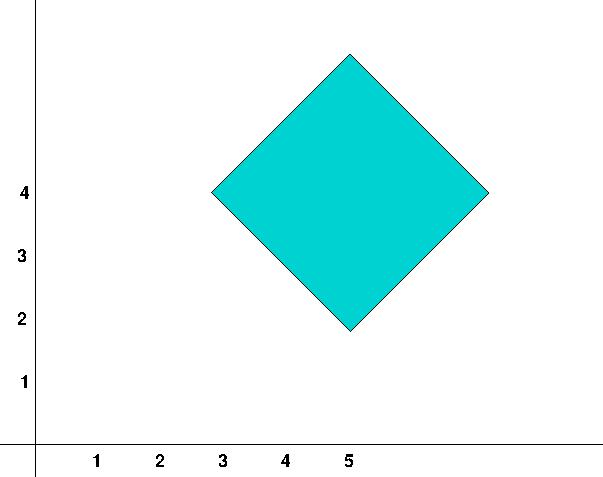
\includegraphics[scale=0.3]{Q3Images/square3.jpg} 
	\centerline{\label{fig1b} \small (1b) Quadrado de lado 3}
\end{minipage}
\end{figure}

%
%
%
\item[{\bf Q4.}] \textbf{Apenas para os alunos de pós-graduação} 
\begin{itemize}
\item Leia o artigo do Torre e do Poggio
  \url{ftp://publications.ai.mit.edu/ai-publications/pdf/AIM-768.pdf}
  e faça um resumo de acordo com as indicações que deixei no
  paca (artigos sobre como fazer um resumo). 
\item O que é um problema mal-posto?
\item O que é regularização? 
\item Qual a importância do teorema apresentado no artigo?
\item O que são filtros de banda limitada? Qual a sua importância no
  artigo?
\item Quais são os métodos de encontrar borda apresentados no artigo?
\end{itemize}
\end{itemize}
\end{document}
